\subsubsection*{Gradient Descent and backpropagation}
Gradient Descent is an algorithm used to find the optimal weights to produce the
smallest prediction error. It is used to overcome problems of non linearly
separable classes. Gradient descent search selects a random weight value and
then modifies it gradually to minimize the error. "At each step, the weight
vector is altered in the direction that produces the steepest descent along the
surface" \parencite{MLANN}. This step is iterated until the lowest value is met.

There is an error function used for the perceptron which finds the lowest error for that neuron, but it can't be used here because, since we have many neurons, there could be an error in multiple neurons.
Gradient Descent is mathematically based on the derivative of a function.
The gradient of a function can be calculated by differentiating it.
As the weights are what is being controlled, " they are what we differentiate in respect to" \parencite{MLAlgorithm}.
The negative gradient of this function is followed to find the lowest possible point, hence the name gradient descent \parencite{MLAlgorithm}.

One problem with Gradient Descent is that if we look at Figure \ref{fig:GD}, we may
never get to the optimal point, point B. This is because we will find point A
without too many problems but when the weights change we will get too high a
slope of error and therefore will never reach point B.

Another variation of Gradient Descent is Stochastic Gradient Descent (SGD). SGD
is different because it updates " weights incrementally, following the
calculation of the error of each individual example" \parencite{MLANN}. 

\begin{figure}[h]
      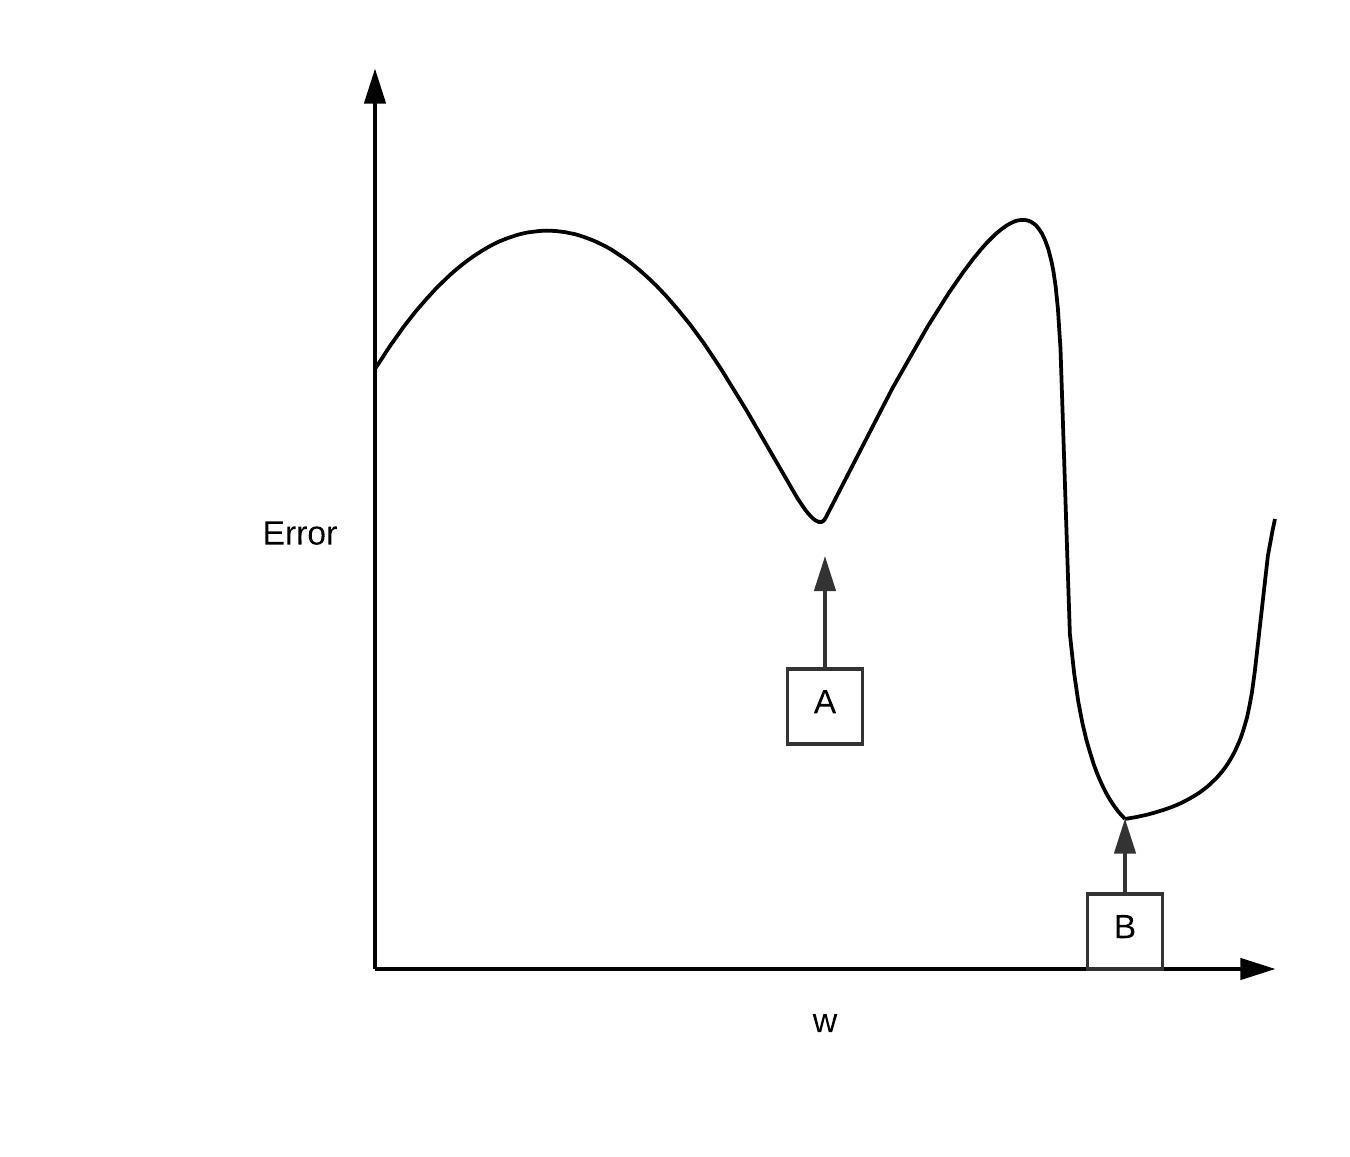
\includegraphics{GradientDescent}
      \caption{Gradient Descent}
      \label{fig:GD}
 \end{figure}

"The Backpropagation algorithm learns the weights of a multilayer network,
given a network with a fixed set of units and interconnections" \parencite{MLANN}.
Backpropagation attempts to minimise the mean squared error between the target
output and the output of a network.

Backpropagation works by starting at the output layer of the network and going
back through previous hidden layers, updating weights as it goes i.e. it propagates back through the network, updating the weights to try and reduce the error.

\parencite{MLANN} defined a walk through of the backpropagation algorithm.
For every value of \[\vec{x}, \vec{t}\], in the training set where x is a vector of inputs and t is a vector of output values to act a target:
\begin{itemize}
	\item{Run x through the network and output \[o_{u}\]}
	\item{For each output k, calculate the error by: \[\delta_{k} \leftarrow o_{k}(1 - o_{k})(t_{k} - o_{k}) \]}
	\item{For every hidden unit, calculate the error by: \[\delta_{h} \leftarrow o_{h}(1 - o_{h}) \sum_{k \in outputs}   w_{kh}\delta_{k}\]}
	\item{Updates weights by: \[w_{ji} \leftarrow w_{ji} + \Delta w_{ji}\] where \[\Delta w_{ji} = \n \delta_{j} x_{ji}\]}
\end{itemize}
